\documentclass[12pt]{book}
\usepackage[polish]{babel}
\let\lll\undefined
\selectlanguage{polish}
\usepackage[utf8]{inputenc}
\usepackage{lmodern}
\usepackage{indentfirst}
\usepackage[plmath]{polski}
\usepackage{icomma}
\frenchspacing
\usepackage{amsmath}
\usepackage{amssymb}
\usepackage{mathrsfs}
\usepackage{bbold}
\usepackage{mathtools}
\usepackage[table]{xcolor}
\usepackage{tabu}
\usepackage{xcolor}
\usepackage{bm}
\definecolor{lgray}{HTML}{9F9F9F}
\definecolor{dgray}{HTML}{5F5F5F}
\usepackage[ruled,vlined,linesnumbered,longend,algochapter]{algorithm2e}
\newenvironment{pseudokod}[1][htb]{
	\renewcommand{\algorithmcfname}{Pseudokod}
	\begin{algorithm}[#1]%
	}{
\end{algorithm}
}
\newcommand\algcomment[1]{
	\footnotesize{#1}
}
\SetCommentSty{algcomment}

\usepackage{textcomp}%
\newcommand{\textapprox}{\raisebox{0.5ex}{\texttildelow}}

% Listowanie kodów źródłowych
\usepackage{listings} 
\renewcommand{\lstlistingname}{Kod źródłowy} % Polska nazwa listingu

% Definicje pecjalnych znaków, które nie są obsługiwane w środowisku listing
\lstset{literate=
	{ż}{{\.{z}}}1	{ź}{{\'{z}}}1
	{ć}{{\'{c}}}1	{ń}{{\'{n}}}1
	{ą}{{\c a}}1	{ś}{{\'{s}}}1
	{ł}{{\l}}1		{ę}{{\c{e}}}1
	{ó}{{\'{o}}}1	{á}{{\'a}}1
	{é}{{\'e}}1		{í}{{\'i}}1
	{ó}{{\'o}}1		{ú}{{\'u}}1
	{ù}{{\`u}}1		{Á}{{\'A}}1
	{É}{{\'E}}1		{Í}{{\'I}}1
	{Ó}{{\'O}}1		{Ú}{{\'U}}1
	{à}{{\`a}}1		{è}{{\'e}}1
	{ì}{{\`i}}1		{ò}{{\`o}}1
	{ò}{{\`o}}1		{À}{{\`A}}1
	{È}{{\'E}}1		{Ì}{{\`I}}1
	{Ò}{{\`O}}1		{Ò}{{\`O}}1
	{ä}{{\"a}}1		{ë}{{\"e}}1
	{ï}{{\"i}}1		{ö}{{\"o}}1
	{ü}{{\"u}}1		{Ä}{{\"A}}1
	{Ë}{{\"E}}1		{Ï}{{\"I}}1
	{Ö}{{\"O}}1		{Ü}{{\"U}}1
	{â}{{\^a}}1		{ê}{{\^e}}1
	{î}{{\^i}}1		{ô}{{\^o}}1
	{û}{{\^u}}1		{Â}{{\^A}}1
	{Ê}{{\^E}}1		{Î}{{\^I}}1
	{Ô}{{\^O}}1		{Û}{{\^U}}1
	{œ}{{\oe}}1		{Œ}{{\OE}}1
	{æ}{{\ae}}1		{Æ}{{\AE}}1
	{ß}{{\ss}}1		{ç}{{\c c}}1
	{Ç}{{\c C}}1	{ø}{{\o}}1
	{å}{{\r a}}1	{Å}{{\r A}}1
	{€}{{\EUR}}1	{£}{{\pounds}}1
}

% ***************************************************************************************************
% Marginesy 
% ***************************************************************************************************

% Ustawienia rozmiarów stron i ich marginesów
\usepackage[headheight=18pt, top=25mm, bottom=25mm, left=25mm, right=25mm]{geometry}
% headheight		-	wysokość tytułów
% top				-	margines górny
% bottom			-	margines dolny
% left				-	margines lewy
% right				-	margines prawy

% Usunięcie górnego marginesu dla środowisk
\makeatletter
\setlength\@fptop{0\p@}	
\makeatother

% ***************************************************************************************************
% Styl 
% ***************************************************************************************************

% Definiuje środowisko 'titlingpage', które zapewnia pełną kontrolę nad układem strony tytułowej.
\usepackage{titling}


% Umożliwia modyfikowanie stylu spisu treści
\usepackage{tocloft}	

\tocloftpagestyle{tableOfContentStyle}

% Definiowanie własnych stylów nagłówków i/lub stopek
\usepackage{fancyhdr}

% Domyślny styl dla pracy 
\fancypagestyle{custom}{
	\fancyhf{}									% wyczyść stopki i nagłówki
	\fancyhead[RO]{								% Prawy, nieparzysty nagłówek
		\hrulefill \hspace{16pt} \large Rozdział \thechapter
		\put(-472.1, 12.1){%
			\makebox(0,0)[l]{%
				
\includegraphics[width=0.05\textwidth]{pwr-logo}
			}
		}
		\put(-443,5.5){%
			\makebox(0,0)[l]{%
				\small Politechnika Wrocławska
			}
		}
	}
	\fancyhead[LE]{								% Lewy, parzysty nagłówek
		\large Rozdział \thechapter \hspace{16pt} \hrulefill 
		\put(-22, 12.1){%
			\makebox(0,0)[l]{%
				
\includegraphics[width=0.05\textwidth]{wppt-logo}
			}
		}
		\put(-240,5.5){%
			\makebox(0,0)[l]{%
				\small Wydział Podstawowych Problemów Techniki
			}
		}
	}
	\fancyfoot[LE,RO]{							% Stopki
		\thepage
	}
	\renewcommand{\headrulewidth}{0pt}			% Grubość linii w nagłówku
	\renewcommand{\footrulewidth}{0.2pt}		% Grubość linii w stopce
}


% Domyślny styl dla bibliografii
\fancypagestyle{bibliographyStyle}{
	\fancyhf{}									% wyczyść stopki i nagłówki
	\fancyhead[RO]{								% Prawy, nieparzysty nagłówek
		\hrulefill \hspace{16pt} \large Dodatek \thechapter
		\put(-472.1, 12.1){%
			\makebox(0,0)[l]{%
				
\includegraphics[width=0.05\textwidth]{pwr-logo}
			}
		}
		\put(-443,5.5){%
			\makebox(0,0)[l]{%
				\small Politechnika Wrocławska
			}
		}
	}
	\fancyhead[LE]{								% Lewy, parzysty nagłówek
		\large Bibliografia \hspace{16pt} \hrulefill 
		\put(-22, 12.1){%
			\makebox(0,0)[l]{%
				
\includegraphics[width=0.05\textwidth]{wppt-logo}
			}
		}
		\put(-240,5.5){%
			\makebox(0,0)[l]{%
				\small Wydział Podstawowych Problemów Techniki
			}
		}
	}
	\fancyfoot[LE,RO]{							% Stopki
		\thepage
	}
	\renewcommand{\headrulewidth}{0pt}			% Grubość linii w nagłówku
	\renewcommand{\footrulewidth}{0.2pt}		% Grubość linii w stopce
}

% Domyślny styl dla dodatków
\fancypagestyle{appendixStyle}{
	\fancyhf{}									% wyczyść stopki i nagłówki
	\fancyhead[RO]{								% Prawy, nieparzysty nagłówek
		\hrulefill \hspace{16pt} \large Dodatek \thechapter
		\put(-472.1, 12.1){%
			\makebox(0,0)[l]{%
				
\includegraphics[width=0.05\textwidth]{pwr-logo}
			}
		}
		\put(-443,5.5){%
			\makebox(0,0)[l]{%
				\small Politechnika Wrocławska
			}
		}
	}
	\fancyhead[LE]{								% Lewy, parzysty nagłówek
		\large Dodatek \thechapter \hspace{16pt} \hrulefill 
		\put(-22, 12.1){%
			\makebox(0,0)[l]{%
				
\includegraphics[width=0.05\textwidth]{wppt-logo}
			}
		}
		\put(-240,5.5){%
			\makebox(0,0)[l]{%
				\small Wydział Podstawowych Problemów Techniki
			}
		}
	}
	\fancyfoot[LE,RO]{							% Stopki
		\thepage
	}
	\renewcommand{\headrulewidth}{0pt}			% Grubość linii w nagłówku
	\renewcommand{\footrulewidth}{0.2pt}		% Grubość linii w stopce
}

% Osobny styl dla stron zaczynających rozdział/spis treści itd. (domyślnie formatowane jako "plain")
\fancypagestyle{chapterBeginStyle}{
	\fancyhf{}%
	\fancyfoot[LE,RO]{
		\thepage
	}
	\renewcommand{\headrulewidth}{0pt}
	\renewcommand{\footrulewidth}{0.2pt}
}

% Styl dla pozostałych stron spisu treści
\fancypagestyle{tableOfContentStyle}{
	\fancyhf{}%
	\fancyfoot[LE,RO]{
		\thepage
	}
	\renewcommand{\headrulewidth}{0pt}
	\renewcommand{\footrulewidth}{0.2pt}
}

% Formatowanie tytułów rozdziałów i/lub sekcji
\usepackage{titlesec}

% Formatowanie tytułów rozdziałów
\titleformat{\chapter}[hang]					% kształt
{
	\vspace{-10ex}
	\Huge
	\bfseries
}												% formatowanie tekstu modyfikowanego elementu
{}												% etykieta występująca przed tekstem modyfikowanego elementu, niewidoczna w spisie treści
{
	10pt
}												% odstęp formatowanego tytułu od lewego marginesu/etykiety
{
	\Huge
	\bfseries
}												% formatowanie elementów przed modyfikowanym tytułem
[
\vspace{2ex}
%\rule{\textwidth}{0.4pt}
%\vspace{-4ex}
]												% dodatkowe formatowanie stosowane poniżej modyfikowanego tytułu


% Formatowanie tytułów sekcji
\titleformat{\section}[hang]					% kształt
{
	\vspace{2ex}
%	\titlerule\vspace{1ex}
	\Large\bfseries
}												% formatowanie tekstu modyfikowanego elementu
{
	\thesection									% etykieta występująca przed tekstem modyfikowanego elementu, niewidoczna w spisie treści
}
{
	0pt
}												% odstęp formatowanego tytułu od lewego marginesu/etykiety
{
	\Large
	\bfseries
}												% formatowanie elementów przed modyfikowanym tytułem

% ***************************************************************************************************
% Linki
% ***************************************************************************************************

% Umożliwia wstawianie hiperłączy do dokumentu
\usepackage{hyperref}							% Aktywuje linki

\hypersetup{
	colorlinks	=	true,					% Koloruje tekst zamiast tworzyć ramki.
	linkcolor		=	blue,					% Kolory: referencji,
        citecolor		=	blue,					% cytowań,
	urlcolor		=	blue					% hiperlinków.
}

% Do stworzenia hiperłączy zostanie użyta ta sama (same) czcionka co dla reszty dokumentu
\urlstyle{same}




% ***************************************************************************************************
% Linki
% ***************************************************************************************************

% Umożliwia zdefiniowanie własnego stylu wyliczeniowego
\usepackage{enumitem}

% Nowa lista numerowana z trzema poziomami
\newlist{myitemize}{itemize}{3}

% Definicja wyglądu znacznika pierwszego poziomu
\setlist[myitemize,1]{
	label		=	\textbullet,
	leftmargin	=	4mm}

% Definicja wyglądu znacznika drugiego poziomu
\setlist[myitemize,2]{
	label		=	$\diamond$,
	leftmargin	=	8mm}

% Definicja wyglądu znacznika trzeciego poziomu
\setlist[myitemize,3]{
	label		=	$\diamond$,
	leftmargin	=	12mm
}

% ***************************************************************************************************
% Inne pakiety
% ***************************************************************************************************

% Dołączanie rysunków
\usepackage{graphicx}

% Figury i przypisy
\usepackage{caption}
\usepackage{subcaption}

% Umożliwia tworzenie przypisów wewnątrz środowisk
\usepackage{footnote}

% Umożliwia tworzenie struktur katalogów
\usepackage{dirtree}

% Rozciąganie komórek tabeli na wiele wierszy
\usepackage{multirow}

% Precyzyjne obliczenia szerokości/wysokości dowolnego fragmentu wygenerowanego przez LaTeX
\usepackage{calc}

% ***************************************************************************************************
% Matematyczne skróty
% ***************************************************************************************************

% Skrócony symbol liczb rzeczywistych
\newcommand{\RR}{\mathbb{R}}

% Skrócony symbol liczb naturalnych
\newcommand{\NN}{\mathbb{N}}

% Skrócony symbol liczb wymiernych
\newcommand{\QQ}{\mathbb{Q}}

% Skrócony symbol liczb całkowitych
\newcommand{\ZZ}{\mathbb{Z}}

% Skrócony symbol logicznej implikacji
\newcommand{\IMP}{\rightarrow}

% Skrócony symbol  logicznej równoważności
\newcommand{\IFF}{\leftrightarrow}

% ***************************************************************************************************
% Środowiska
% ***************************************************************************************************

% Środowisko do twierdzeń
\newtheorem{theorem}{Twierdzenie}[chapter]

% Środowisko do lematów
\newtheorem{lemma}{Lemat}[chapter]

% Środowisko do przykładów
\newtheorem{example}{Przykład}[chapter]

% Środowisko do wniosków
\newtheorem{corollary}{Wniosek}[chapter]

% Środowisko do definicji
\newtheorem{definition}{Definicja}[chapter]

% Środowisko do dowodów
\newenvironment{proof}{
	\par\noindent \textbf{Dowód.}
}{
\begin{flushright}
	\vspace*{-6mm}\mbox{$\blacklozenge$}
\end{flushright}
}

% Środowisko do uwag
\newenvironment{remark}{
	\bigskip \par\noindent \small \textbf{Uwaga.}
}{
\begin{small}
	\vspace*{4mm}
\end{small}
}
\hyphenation{wszy-stkich ko-lu-mnę każ-da od-leg-łość
	dzie-dzi-ny dzie-dzi-na rów-nych rów-ny
	pole-ga zmie-nna pa-ra-met-rów wzo-rem po-cho-dzi
	o-trzy-ma wte-dy wa-run-ko-wych lo-gicz-nie
	skreś-la-na skreś-la-ną cał-ko-wi-tych wzo-rów po-rzą-dek po-rząd-kiem
	przy-kład pod-zbio-rów po-mię-dzy re-pre-zen-to-wa-ne
	rów-no-waż-ne bi-blio-te-kach wy-pro-wa-dza ma-te-ria-łów
	prze-ka-za-nym skoń-czo-nym moż-esz na-tu-ral-na cią-gu tab-li-cy
	prze-ka-za-nej od-po-wied-nio}
\frontmatter

\begin{document}

	\begin{titlingpage}
		\vspace*{\fill}
		\begin{center}
			\begin{picture}(300,510)
				\put(11,520){\makebox(0,0)[l]{\large \textsc{Wydział Podstawowych Problemów Techniki}}}
				\put(11,500){\makebox(0,0)[l]{\large \textsc{Politechnika Wrocławska}}}
% Tytuł pracy
				\put(80,320){\Huge \textsc{Systemy rekomendacji}}
				\put(80,280){\Huge \textsc{oparte na}}
				\put(80,240){\Huge \textsc{błądzeniu losowym}}
% Autor pracy
				\put(90,200){\makebox(0,0)[l]{\large \textsc{Piotr Kasprowicz}}}
				\put(90,180){\makebox(0,0)[l]{\large \textsc{Nr indeksu: 236609}}}

				\put(200,100){\makebox(0,0)[l]{\large Praca inżynierska napisana}}
				\put(200,80){\makebox(0,0)[l]{\large pod kierunkiem}}
% dane promotora
				\put(200,60){\makebox(0,0)[l]{\large dra inż. Jakuba Lemiesza}}
				
				\put(115,-70){
\includegraphics[width=0.15\textwidth]{pwr}}
				\put(106,-80){\makebox(0,0)[bl]{\large \textsc{Wrocław 2019}}}
			\end{picture}
		\end{center}	
		\vspace*{\fill}
	\end{titlingpage}
	
        \cleardoublepage
		
	\pagenumbering{Roman}
	\pagestyle{tableOfContentStyle}
	\tableofcontents
	\cleardoublepage
		
	% ***************************************************************************************************
	% Wstęp
	% ***************************************************************************************************
	
	\pagestyle{custom}
	\mainmatter
	
	% ***************************************************************************************************
	% Rodziały
	% ***************************************************************************************************

	\chapter{Wstęp}
\thispagestyle{chapterBeginStyle}

We współczesnym nam świecie istnieje ciągła potrzeba tworzenia ofert i polecania produktów różnym klientom. Proste mechanizmy takie jak lista bestsellerów w księgarni internetowej, czy lista nowych produktów w sklepie z odzieżą stają się niewystarczające. Celem zwiększenia swoich szans w walce z konkurencją oraz zmaksymalizowania dochodów serwisy internetowe zaczęły rozglądać się za sposobem na ustalenie gustu indywidualnego klienta.

Z pomocą przyszły systemy rekomendacji, które pozwalają na stworzenie oferty spersonalizowanej pod wybranego użytkownika. Sprawdziły się one w swoim zadaniu tak efektywnie, że korzysta z nich większość serwisów internetowych. W branży e-handlu (ang. \textit{e-commerce}) Amazon stał się liderem sprzedaży stosując takie systemy przy polecaniu aukcji, serwisy hostujące wideo oraz muzykę np. Youtube czy Spotify nie byłyby tak efektywne w proponowaniu kolejnych filmów czy utworów, a wyszukiwanie znajomych na portalu społecznościowym takim jak Facebook, który w sierpniu 2019 roku przekroczył 2.45 miliarda aktywnych użytkowników \cite{facebook} byłoby po prostu niemożliwe.

Główną ideą stojącą za silnikami rekomendacji jest znalezienie pewnego podobieństwa między użytkownikiem, a produktami lub innymi użytkownikami, a następnie stworzenie rankingu, który je porówna. Ponieważ są one tak szeroko wykorzystywane, istnieje wielu różnych podejść oraz implementacji. Dwa główne, które możemy wyróżnić to metoda Content-based filtering, która polega na polecaniu produktów na podstawie tego, czym użytkownik interesował się w przeszłości oraz metoda Collaborative filtering, w której przy rekomendacji wykorzystujemy informacje jakie produkty podobały się użytkownikom o podobnym guście \cite{RecommenderASurvey}. Wszelkie inne stanowią najczęściej kombinacje obu technik z zamiarem dopasowania systemu do konkretnego problemu.
%JL lub rozwiązania problemu dotykającą, którąś z powyższych koncepcji.

Celem pracy jest porównanie technik wykorzystywanych do tworzenia systemu rekomendacji, a następnie stworzenie takiego systemu 
%JL w oparciu o błądzenie losowe 
w kontekście problemu przydzielania recenzentów do oceniania prac naukowych.

Praca składa się z czterech rozdziałów.
W rozdziale pierwszym znajduje się opis oraz klasyfikacja systemów rekomendacji, 
a w szczególności wprowadzenie do techniki opartej na spacerach losowych.


W rozdziale drugim przedstawiono opis stworzonego systemu.

W rozdziale trzecim znajduje się testy zaimplementowanego systemu.

W rozdziale czwartym przedstawiono sposób instalacji i wdrożenia systemu w środowisku docelowym.

Końcowy rozdział stanowi podsumowanie uzyskanych wyników.
	\cleardoublepage

	\chapter{Systemy rekomendacji}
\thispagestyle{chapterBeginStyle}

\section{Rodzaje systemów rekomendacji}

Systemy rekomendacji to rodzaj filtrów informacji, które powstały w celu odnalezienia w zbiorze danych produktu, który trafi w osobiste preferencje użytkownika. Występują one w całym Internecie rozpowszechnione za sprawą wyszukiwarek internetowych, dla których początkowo powstały. Jednym z pierwszych takich miejsc, w którym możemy się na nie natknąć pojawia się przy okazji autouzupełniania (ang. \textit{autocomplete}) wpisywanego tekstu. Naturalne stało się to, że nowoczesne narzędzia tworzą dla nas podpowiedzi, co dzieje się na podstawie częstotliwości wpisanych fraz przez innych użytkowników oraz historii naszych wcześniejszych wyszukań. W ten sposób pomagają one uniknąć takich pomyłek jak błędy ortograficzne czy literówki. Dodatkowo, zastosowanie takiego mechanizmu w wyszukiwarce internetowej ułatwia jej udzielenie poprawnej odpowiedzi na stworzone zapytanie, poprzez zaproponowanie specjalistycznego słownictwa lub synonimu, który lepiej pasuje w danym kontekście. Przechodząc do wyszukiwarek natrafiamy na kolejny przykład wykorzystania naszych systemów, a mianowicie globalne systemy rankingowe, czyli sposób na ocenę i pozycjonowanie wszystkich stron internetowych w wynikach wyszukiwania. Idea działania algorytmu PageRank (wykorzystanego m.in. w przeglądarce Google) została opisana w dalszej części pracy, w rozdziale poświęconemu temu zagadnieniu.

Zastosowaniem, na którym skupiamy się w tej pracy jest personalizacja wyników pod konkretnych użytkowników (w skrócie PRES, z ang. \textit{Personalized Recommender System}). Takie silniki rekomendacji znajdują swoje zastosowanie głównie w komercyjnych rozwiązaniach, gdzie odpowiednia propozycja może w znaczący sposób zachęcić użytkownika do ponownego skorzystania z serwisu. Najpopularniejsze aplikacje tych systemów to generowanie playlist dla serwisów wideo oraz muzyki jak Youtube i Netflix, tworzenie preferencyjnych ofert dla użytkowników aukcji internetowych takich jak Amazon czy Allegro lub tworzenie dla portali społecznościowych jak Facebook czy Twitter powiązań między użytkownikami. Ze względu na różnice w implementacji możemy rozpatrzyć 3 różne podejścia:
\begin{itemize}
    \item metoda content-based,
    \item metoda collaborative filtering,
    \item metoda hybrydowa, która łączy dwie pierwsze podejścia.
\end{itemize}

\begin{figure}[h]
    \centering
    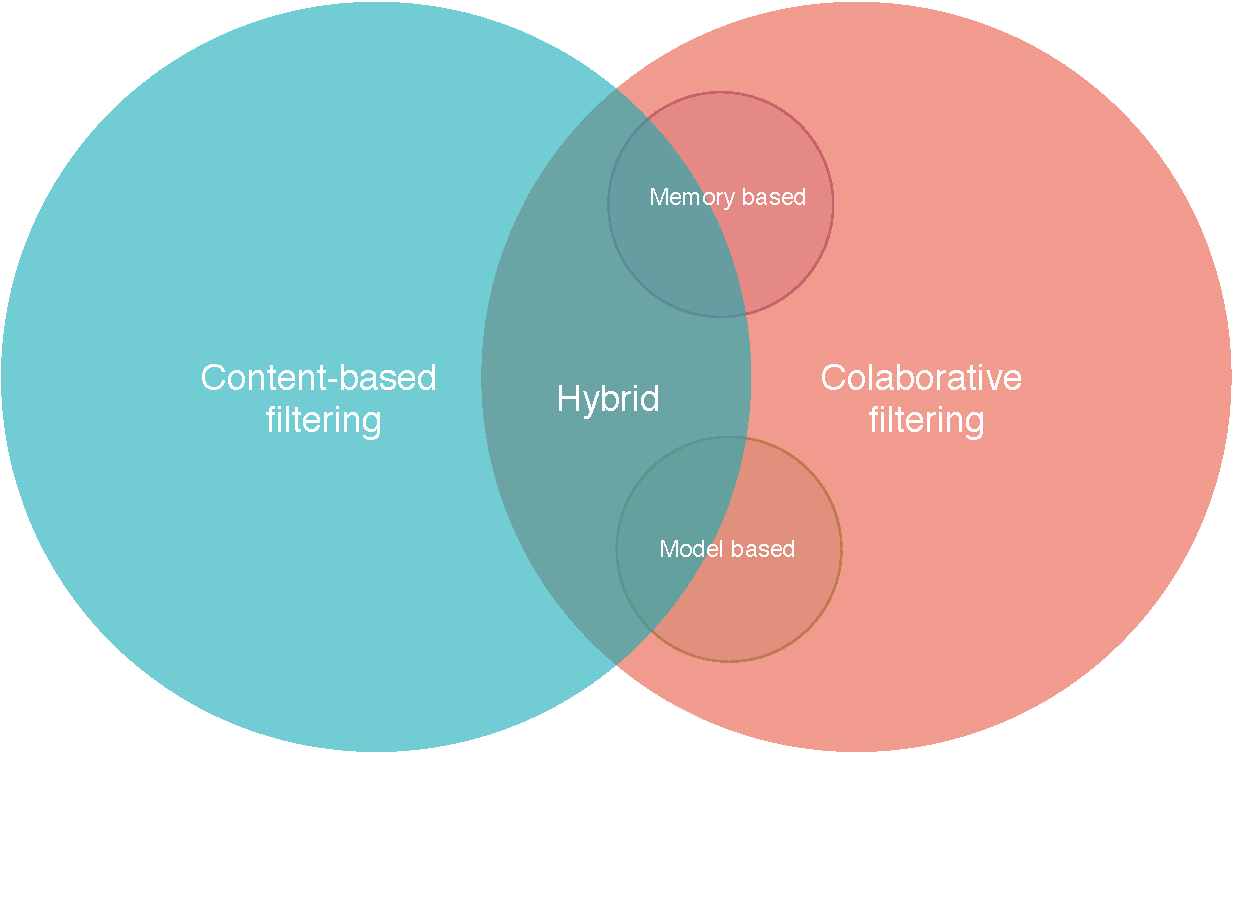
\includegraphics[width=\textwidth]{data/Venn.pdf}
    \caption{Podział systemów rekomendacji}
    \label{fig:my_label}
\end{figure}

\section{Gromadzenie informacji}

Zanim przejdziemy do opisu metod tworzenia rankingu, musimy w jakiś sposób zebrać dane o użytkowniku, aby poznać jego preferencje. W tym celu zasadniczo korzysta się dwóch źródeł informacji, z jawnej (ang. explicit feedback) lub domniemanej  (ang. implicit feedback) informacji zwrotnej. Pierwszą uzyskujemy poprzez przeprowadzenie ankiety na nowo stworzonym koncie w celu bezpośredniego uzupełnienia informacji o interesujących nas cechach na podstawie odpowiedzi jakie zostały udzielone. Tak uzyskane informacje mogą pozytywnie wpłynąć na modelowanie użytkownika oraz generowanie rekomendacji:
\begin{itemize}
    \item Po pierwsze pomagają w rozwiązaniu problemu braku gęstości danych (ang. \textit{large data sparesity}) poprzez wymuszenie dodatkowych informacji o preferencjach użytkownika, a co za tym idzie zwiększenie liczby relacji między obiektami w systemie.
    \item Po drugie rozwiązuje cold-start problem, na który napotykamy w systemach rekomendacji w momencie, gdy rejestruje się nowy użytkownik i nie mamy o nim żadnych informacji. W tym problemie rozróżniamy dwa rodzaje użytkowników: pierwszy, który miał małą styczność z obiektami w systemie oraz drugi, który jest całkowicie nowy dla systemu. Dla pierwszego typu ankieta może zostać wykorzystana do wzmocnienia oceny atrybutów w profilu użytkownika, a dla drugiego do stworzenia takiego profilu oraz polepszenia jakości całego rankingu.
    \item Trzecią korzyścią płynąca z zastosowania ankietyzacja użytkowników dla modeli, które nie mierzą się z problemem małej ilości danych jest ustalenie jakości stworzonego rankingu poprzez porównanie go z odpowiedziami udzielonymi w ankiecie oraz rozpoznanie ukrytych preferencji użytkownika, które nie zostały wykryte innymi metodami. \cite{RecommenderSystemsBasedonUserReviews:TheStateoftheArt}
\end{itemize}

Portale na których pobierana jest informacja od użytkownika (np. Twitter oraz Pintrest) czerpią ogromne korzyści z możliwości wyświetlania dostosowanej do niego zawartości. 
Zaraz po rejestracji użytkownik proszony jest o ocenę jakie treści go interesują w celu zapewnienia spersonalizowanych rekomendacji. W ten sposób, o ile ankietowany nie skłamał w odpowiedziach, możemy zaprezentować mu treści pasujące do jego upodobań.

Drugim rozwiązaniem jest wykorzystanie wcześniejszych zachowań lub wyborów użytkownika. Można wykorzystać np. wcześniej wybrany przez niego przedmiot lub czas jaki spędzi podczas przeglądania oferty. Zbieraniem informacji o jego działaniach zajmuje się system, który monitoruje każdy jego ruch. Implementacja tego podejścia jest o wiele bardziej skomplikowana, dlaczego często łączona jest z pierwszą, na przykład w serwisie YouTube przy rekomendacji filmów wykorzystywana jest informacja jawna o tym które kanały zostały przez użytkownika zasubskrybowane i polubione, oraz dodatkowo zbierane są informacje o tym, które filmy zostały przez niego obejrzane w całości, a z oglądania których zrezygnował po kilku minutach.

Popularną metodą wykorzystywaną do wydobycia ważnych z punktu widzenia systemu informacji o użytkowniku bez jego aktywnego zaangażowania, używany w 83\% biblotek cyfrowych \cite{Research-paperrecommendersystems:aliteraturesurvey} jest indeks \textit{tf-idf} (ang. term frequency–inverse document frequency). Tradycyjnie wykorzystany jest on do analizy dokumentów tekstowych i umożliwia wskazanie słów najbardziej charakterystycznych dla danego dokumentu, w kontekście większego zbioru dokumentów. Jego pierwszym krokiem jest pozbycie z dokumentów tagów oraz słów, które nie zapewniają istotnych informacji np. znaków interpunkcyjnych oraz często występujących słów. Kolejno z pozostałego zbioru usuwane są prefisy i sufixy w celu odnalezienia podstawowej formy słowa. Następnie bazując na tym jak użytkownik ocenił treść (jawny lub bierny sposób uzyskiwania informacji o preferencjach użytkownika) wybieramy te słowa (termy), które są z punktu widzenia użytkownika interesujące wykorzystując w tym celu wzór na wartość tf-idf:
\begin{equation}
\label{tfidf}
        \mathrm{(tf\text{-}idf)_{i,j}} = \mathrm{tf_{i,j}} \times \mathrm{idf_i},
\end{equation}
gdzie:
\begin{itemize}
    \item $tf_{i, j}$to tzw. „term frequency”, wyrażana wzorem:
\end{itemize}
\begin{equation*}
    \mathrm{tf_{i,j}} = \frac{n_{i,j}}{\sum_k n_{k,j}},
\end{equation*}
gdzie: 
\begin{itemize}
    \item $n_{i,j}$ jest liczbą wystąpień termu $(t_i)$ w dokumencie $d_j,$ a mianownik jest sumą liczby wystąpień wszystkich termów w dokumencie $d_j.$
    \item $idf_{i}$ to „inverse document frequency” wyrażana wzorem:
\end{itemize}
\begin{equation*}
    \mathrm{idf_i} = \log \frac{|D|}{|\{d: t_i \in d\}|},
\end{equation*}
gdzie:
\begin{itemize}
    \item $|D|$ – liczba dokumentów w korpusie,
    \item $|\{d : t_i \in d\}|$ – liczba dokumentów zawierających przynajmniej jedno wystąpienie danego termu.

\end{itemize}

\section{Content-based filtering}
\label{chap:content}


Metoda content-based filtering (CB) rekomenduje użytkownikowi produkty na podstawie utworzonego profilu użytkownika. To podejście najlepiej sprawdza się w sytuacji, gdy znamy dokładne informacje o produkcie (nazwa, lokalizacja, opis), ale mamy niewiele informacji o użytkowniku.

Na początku zarówno dla przedmiotów jak i użytkowników tworzymy profil, typowo reprezentowany za pomocą wektora $X=(x_{1},x_{2},...,x_{n})$, gdzie $x_{n}$ reprezentuje pewną cechę lub atrybut. Następnie porównując wektory za pomocą różnych metryk, możemy obliczyć odległości między nimi i stworzyć ranking, który pozwoli na wybranie przedmiotów podobnych do wektora użytkownika. W rezultacie otrzymujemy listę przedmiotów, które powinny pokryć się z upodobaniami użytkownika.

Jedną z takich miar używanych w przypadku, kiedy rozpatrywane wektory są binarne (wektor składa się z samych zer i jedynek) jest odległość Hamminga. Jej wartość dla dwóch ciągów tej samej długości to liczba pozycji, na których ciągi mają różne wartości. 
W przypadku, gdy wektory składają się z liczb rzeczywistych typowo wykorzystuje się odległość euklidesową \cite{Similarityandrecommendersystems}.
Jeśli w kartezjańskim układzie współrzędnych $\mathbf{a}=(a_1,a_2,...,a_n)$ i $\mathbf{b}=(b_1,b_2,...,b_n)$ są dwoma punktami w n-wymiarowej przestrzeni euklidesowej to odległość (d) między $\mathbf{a}$ i $\mathbf{b}$ lub $\mathbf{b}$ i $\mathbf{a}$ wynosi:
\begin{equation}
    \begin{aligned}
        d(\mathbf{a},\mathbf{b}) = d(\mathbf{a},\mathbf{b}) & = \sqrt{(a_1-b_1)^2 + (a_2-b_2)^2 + \cdots + (a_n-b_n)^2} \\
& = \sqrt{\sum_{i=1}^n (a_i-b_i)^2}.
    \end{aligned}
\end{equation}

Zauważmy w tym miejscu dodatkowo, że w przypadku porównania przedmiotów (ang. \textit{item-to-item}) najczęściej wykorzystywana jest jedna z dwóch następujących miar odległości:
\begin{itemize}
    \item odległość kosinusowa, czyli kosinus kąta między dwoma wektorami reprezentującymi dwóch użytkowników lub dwa produkt \cite{Eksploracjatekstu}. Jego wartość $\cos(\theta)$ obliczana jest następująco:
    \begin{equation}
        \cos(\theta) = {\mathbf{a} \cdot \mathbf{b} \over \|\mathbf{a}\| \|\mathbf{b}\|} = \frac{ \sum\limits_{i=1}^{n}{a_i  b_i} }{ \sqrt{\sum\limits_{i=1}^{n}{a_i^2}}  \sqrt{\sum\limits_{i=1}^{n}{b_i^2}} }~.
    \end{equation}
    Wykorzysywana jest ona miedzy innymi w sklepie internetowym Amazon \cite{Amazon.comRecommendationsItem-to-ItemCollaborativeFiltering}.
    \item Indeks Jaccarda, zdefiniowana jako moc części wspólnej zbiorów $A$ i $B$ przez moc ich sumy, mierzy podobieństwo pomiędzy dwoma zbiorami:
    \begin{equation}
       J (A,B) = \frac{|A \cap B|}{|A \cup B|}.
    \end{equation}
    Podobnie jak odległość Hamminga współczynnik podobieństwa Jaccarda znajduje swoje zastosowanie w systemach rekomendacji w sytuacji, gdy wektory reprezentowane są poprzez wartości binarne.
\end{itemize}

Dzięki zastosowaniu jednej z powyżej opisanych miar odległości jesteśmy w stanie ustalić odległość między wektorami. Jednakże, aby dane były gotowe do porównania i analizy, często wymagają dodatkowych zabiegów. Dla przykładu rozważmy system rekomendacji do rekomendacji filmów i dwóch użytkowników tego systemu, z których jeden konsekwentnie ocenia wyżej niż drugi (zawyża oceny). Odległość między tymi użytkownikami może być duża. Z tego powodu 
typowo stosuję się normalizację ocen, doprowadzając wektory do tzw. postaci standardowej \cite{Similarityandrecommendersystems}.
Niech wektor $x_u = (x_{u1}, x_{u2}, ... , x_{uN})$ opisuje użytkownika $u$, gdzie $x_{un}$ jest jego oceną produktu $n$. Obliczamy średnią ocenę $\overline{x}_{u}$ oraz odchylenie standardowe $s_{u}$ w następujący sposób:
\begin{equation}
\label{eqn:normalizacja1}
     \overline{x}_{u} = \frac{1}{N}\sum_{n=1}^N x_{un}~,
\end{equation}
\begin{equation}
\label{eqn:normalizacja2}
    s_{u} = \sqrt{\frac{1}{N-1} \sum_{n=1}^N(x_{un} - \overline{x}_{u})^2}~.
\end{equation}
Następnie zmieniamy zmienną niestandaryzowaną $x_{un}$ na:
\begin{equation}
\label{eqn:normalizacja3}
    z_{un}= \frac{x_{un}-\overline{x}_{u}}{s_{u}}~.
\end{equation}

System rekomendacji oparty na technice content-based filtering, po obliczeniu podobieństwa pomiędzy przedmiotami a użytkownikami tworzy listę najlepszych rekomendacji. Jeśli niepożądane jest, aby użytkownikowi został polecany produkt, który jest mu już znany, systemu usuwa te pozycje, a następnie prezentuje wynik użytkownikowi. Wadą content-based filtering jest potrzeba wydobycia charakterystycznych cech z przedmiotu, co nie zawsze jest łatwe lub wykonalne. Jeśli przedmiot posiada opis tekstowy, z którego możemy uzyskać informacje
(na przykład wykorzystując indeks tf-idf), wtedy metoda content-based zadziała. Jednakże problem napotykamy w np. momencie w przypadku prób rekomendacji muzyki lub obrazu, gdyż najczęściej nie istnieje łatwy sposób na stworzenie ich matematycznej reprezentacji.

\section{Collaborative filtering}

Druga z metoda stosowanych w systemach rekomendacji to collaborative filtering (CF).
Bazuje ona na pomyśle, że użytkownikom o podobnych upodobaniach odpowiadają podobne produkty. W tym przypadku nie wykorzystujemy charakterystyki produktów, upodobania użytkownika są określane na podstawie jego historii z produktami np. jakie produkty kupił, a następnie na tej podstawie obliczane są korelacje między użytkownikami. Następnie te korelacje służą do stworzenia dopasowania produktów dla konkretnego użytkownika.

Wśród algorytmów rekomendacji wykorzystujących collaborative filtering wyróżniamy 2 podgrupy:
\begin{itemize}
    \item metody wykorzystujące pamięć,
    \item metody wykorzystując model.
\end{itemize}

\subsection{Metody wykorzystujące pamięć}
W metodach wykorzystujące pamięć ponownie można wydzielić 2 typy ze względu na to jakie dane przetwarzają: filtracja użytkownik-produkt (ang. \textit{user-item filtering}) oraz filtracja produkt-produkt (ang.\textit{item-item filtering}).
Przykładem aplikacji filtracji użytkownik-produkt jest algorytm klasyfikacji K najbliższych sąsiadów, który znajduje grupy użytkowników o podobnych zainteresowaniach. Przepływ pracy w tym przypadku standardowo przebiega w 3 krokach:
\begin{itemize}
    \item Użytkownik ocenia dany produkt. Może to się dokonać tak samo jak w poprzedniej metodzie w sposób jawny (ang. \textit{explicit feedback}) lub bierny (ang. \textit{implicit feedback}). Pierwszy polega na bezpośredniej ocenie produktu przez uzytkownika, a drugi na analizie jego zachowań.
    \item System porównuje ocenę produktów użytkownika z oceną innych użytkowników i na tej podstawie wyszukuje tych, którzy mają podobne upodobania jak ten dla którego tworzymy rekomendacje.
    \item Na końcu system rekomenduje przedmioty, które użytkownicy o podobnym guście ocenili wysoko, lecz nie zostały one jeszcze ocenione przez tego użytkownika.
\end{itemize}


Z kolei w przypadku filtracji produkt-produkt cały proces przebiega w następujący sposób:


\begin{itemize}
    \item Ocena produktów przez użytkownika przebiega identycznie jak w filtracji użytkownik-produkt,
    \item Utworzona zostaje macierz reprezentująca relacje między każdą parą przedmiotów.
    \item Na końcu system na wyszukuje w macierzy te przedmioty, które podobały sie użytkownikowi, na tej podstawie odszukuje tych użytkowników, których lubili te przedmioty i zwraca inne produkty, które lubili.
\end{itemize}
Podsumowując w pierwszym przypadku dane wejściowe to użytkownicy, a dane wyjściowe to produkty, a w drugim zarówno dane wejściowe jak i wyjściowe stanowią produkty. W skrócie filtracja użytkownik-produkt może zostać opisana jako “Użytkownikom podobnym do ciebie również podobało się...”, a filtracja produkt-produkt “Użytkownicy, którzy polubili ten produkt również polubili...”.

Podobnie jak przy metodzie content-based, podobieństwo obliczane jest za pomocą odpowiednich miar. Do tego celu wykorzystywana jest opisana już wcześniej odległość kosinusowa lub bardziej popularny w przypadku collaborative filtering współczynnik korelacji Pearsona. Do oszacowania korelacji między ocenami po pierwsze normalizujemy je przy korzystaniu wzorów \eqref{eqn:normalizacja1}, \eqref{eqn:normalizacja2} i \eqref{eqn:normalizacja3} do postaci standardowej, następnie obliczamy korelacje miedzy użytkownikami $x$ i $y$ według następującego wzoru:
\begin{equation}
\begin{aligned}
        r_{xy} & =\frac{1}{N-1} \sum ^N _{n=1} \left( \frac{x_n - \bar{x}}{s_x} \right) \left( \frac{y_n - \bar{y}}{s_y} \right) \\
        & = \frac{1}{N-1} \sum ^N _{i=n} z_{xn} z_{yn}
\end{aligned}
\end{equation}
gdzie:
\begin{itemize}
    \item N - wymiar wektora $x$ oraz $y$,
    \item $x_u = (x_{u1}, x_{u2}, ... , x_{uN})$, opisuje użytkownika $u$, gdzie $x_{un}$ jest oceną produktu n, analogicznie dla $y$,
    \item $\overline{x}$, $\overline{y}$ - średnia dla próby,
    \item $s_x$, $s_y$ - odchylenie standardowe.
\end{itemize}

Korelację można interpretować w następujący sposób: jeśli $z_{xn}$ jest duże, gdy $z_{yn}$ jest duże oraz, gdy $z_{xn}$ jest małe, gdy $z_{yn}$ jest małe wynik korelacji będzie zmierzał do $1$. Jeśli  $z_{xn}$ jest duże, gdy $z_{yn}$ jest małe oraz, gdy $z_{xn}$ jest duże, gdy $z_{yn}$ jest małe wynik korelacji będzie zmierzał do $-1$. W przypadku braku korelacji między użytkownikami wynik korelacji wynik będzie zmierzał do $0$ \cite{Similarityandrecommendersystems}.

\subsection{Metody wykorzystujące model}
Drugie podejście (ang. \textit{model-based collaborative filtering}) polega na stworzeniu rankingu w oparciu o pewien wybrany model.
Przy wykorzystaniu collaborative filtering napotykamy na różnego rodzaju problemy, których kilka opisujemy poniżej.   
Najistotniejsze problemy to brak gęstości danych (ang. data sparsity) i problem skalowalności, które wynikają z tego, że większość komercyjnych systemów rekomendacji jest oparta na wielkich bazach danych. Przez to macierze opisujące relacje między użytkownikiem a produktami i czas wykonywania operacji na takich macierzach rosną do bardzo dużych rozmiarów. Dla przykładu, w serwisie Twitter stosowane są techniki redukcji nieistotnych połączeń oraz dzielenie użytkowników na wiele grup dzięki czemu możliwe jest zastosowanie architektury umożliwiającej  wykonanie obliczeń w klastrze (trwają one wiele miesięcy)  \cite{WTF:TheWhotoFollowServiceatTwitter}.
W takich scenariuszach stosuje się techniki takie jak naiwny klasyfikator bayesowski, analiza skupień (ang. clustering models), przetwarzanie języka naturalnego (ang. \textit{latent semantic analysis}) czy też procesy decyzje Markowa.


Kolejny problem związany z brakiem gęstości danych jest tzw. zimny start (ang. \textit{cold start}). Napotykamy na niego w momencie pojawienia się w systemie nowego użytkownika lub produktu. Taki użytkownik, który nie ocenił produktów lub nowy produkt który nie został jeszcze oceniony wystarczającą ilość razy nie może być odpowiednio wdrożony do systemu. 
Tego rodzaju obiekt nazywa jest ,,czarną owcą'', gdy niemożliwe jest dopasowanie rekomendacji lub ,,szarą owcą'', gdy rekomendacje dla danego obiektu nie są konsekwentne. Ponieważ ten problem nie pojawia się w podejściu content-based  (w której mamy dostępny wektor ustalonych cech) często łączy się obie metody. Takie hybrydowe podejście nazywa się content-boosted collaborative filtering. 

Kolejnym wyzwaniem jest problem długiego ogona (ang. \textit{long tail}), który pojawia się w przypadku gdy większość użytkowników otrzymuje jako rekomendacje, tylko nieznaczna ilość przedmiotów w systemie.

\begin{figure}[h]
    \centering
    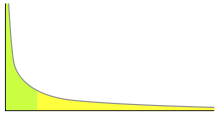
\includegraphics[width=0.4\textwidth]{longtail.png}
    \caption{Zobrazowanie problemu długiego ogona (źródło: \cite{WikipediaEN:Longtail}). Po prawej (żółty kolor) znajduje się długi ogon, po lewej (zielony kolor) reprezentuje małą grupę produktów, które dominują w rekomendacjach.}
    \label{fig:longtail}
\end{figure}


\section{Spacery losowe}
\label{chap:spacerylosowe}

System rekomendacji zaproponowany w tej pracy oparty jest na spacerach losowych. Poniżej przypominamy pojęcia związane ze spacerami losowymi zaczynając od pojęcia procesu stochastycznego i łańcucha Markowa. Proces stochastyczny definiujemy jako rodzinę zmiennych losowych $\mathbf{X}=\{X(t): t \in T\}$. Oznaczenie $X(t)$ lub $X_t$ rozumiemy jako stan procesu w czasie $t$. 
Będziemy dalej rozpatrywać procesy z czasem dyskretnym i skończone (tzn. zmienne $X_t$ będą przyjmować wartości ze zbioru skończonego). Łańcuch Markowa definiujemy następująco:

\begin{definition}\label{def:markow}
Jednorodny proces stochastyczny z czasem dyskretnym $X_{0}, X_{1}, X_{2},\dots$ jest łańcuchem Markowa, jeśli \cite{Metodyksiazka}

\begin{equation}
\begin{aligned}
    Pr(X_{t}= a_{t} | X_{t-1} = a_{t-1}, X_{t-2} = a_{t-2},\dots, X_{0} = a_{0}) = & Pr(X_{t} = a_{t} | X_{t-1} = a_{t-1}) = \\ & P_{a_{t-1},a_{t}} .
\end{aligned}
\end{equation}
\end{definition}

Z powyższej definicji wynika fakt nazywany własnością Markowa lub własność braku pamięci, który mówi o tym stan $X_{t}$ zależy wyłącznie od poprzedniego stanu, a nie w jaki sposób w naszym procesie dotarliśmy do stanu $X_{t-1}$. Jednakże należy pamiętać, że nie oznacza to, że w procesie o własności Markowa zmienna $X_{t}$ jest niezależna od zmiennych losowych $X_{0},X_{1},\dots,X_{t-2}$.
Oznacza to jedynie, że zależność $X_t$ od przeszłości jest zawarta w $X_{t-1}$ \cite{Metodyksiazka}.

Z tej własności wynika fakt, że proces Markowa jest jednoznacznie zdefiniowany przez macierz przejść w jednym kroku
\begin{equation*}
\bm{P} =
\left(\begin{array}{ccccc}
P_{0,0} & P_{0,1}  & \cdots & P_{0,j} & \cdots \\
P_{1,0} & P_{1,1}  & \cdots & P_{1,j} & \cdots \\
\vdots & \vdots & \ddots & \vdots & \ddots \\
P_{i,0} & P_{i,1}  & \cdots & P_{i,j} & \cdots \\
\vdots & \vdots & \ddots & \vdots & \ddots \\
\end{array}\right) .
\label{eq:postac}
\end{equation*} 

W związku z tym, że wyraz w i-tym wierszu i j-tej kolumnie jest prawdopodobieństwem tego, że proces przechodzi z i do j w jednym kroku, wynika że dla każdego i, $\sum_{j\ge0} P_{i,j}=1$ \cite{Metodyksiazka}. Tę reprezentację można w wygodny sposób wykorzystać do obliczeń kolejnych stanów procesu. Jeśli $\overrightarrow{p}(t)=(p_0(t),p_0(t),p_0(t),\dots )$  będzie wektorem określającym dystrybucję stanu łańcucha w czasie $t$, gdzie $p_i(t)$ oznacza, że proces znajduje sie w stanie $i$ w czasie $t$, to kolejne kroki obliczamy iterując nastepujące równanie:
\begin{equation}
    \overrightarrow{p}(t)=\overrightarrow{p}(t-1)\bm{P}.
\end{equation}


Spacer losowy (lub inaczej błądzenie losowe) to nieskomplikowany proces stochastyczny, który często odbywa się na prostej, na płaszczyźnie lub na grafie. W tej pracy rozważamy spacery odbywające się na grafach.
\begin{definition}[Spacer losowy na grafie \cite{Metodyksiazka}]\label{def:spacer}
Spacer losowy na grafie G jest łańcuchem Markowa zdefiniowanym przez ciąg ruchów cząsteczki między wierzchołkami grafu G. W tym łańcuchu stan spaceru odpowiada położeniu cząsteczki w danym kroku. Jeśli cząsteczka jest w wierzchołku $i$, który ma $d(i)$ krawędzi, to prawdopodobieństwo, że cząsteczka będzie poruszać wzdłuż krawędzi $(i, j)$ i przejdzie do sąsiedniego wierzchołka $j$ jest równe $1/d(i)$ .
\end{definition}

Wykorzystanie błądzenia losowego w systemach rekomendacji to wygodny sposób na przedstawienie relacji mogących być wykorzystanych w celu stworzenie rekomendacji. Systemy oparte o błądzenie losowe są w dużej mierze odporne na takie problemy jak małą gęstość danych i dobrze sprawdzają się przy dużych zbiorach danych. Ze względu na różne zastosowania możemy podzielić je na \cite{RecommenderASurvey} :
\begin{itemize}
    \item globalne systemy rankingowe,
    \item spacery losowe z restartami,
    \item absorbujące spacery losowe.
\end{itemize}


\section{Globalne systemy rankingowe}


Globalne systemy rankingowe wykorzystują błądzenie losowe do stworzenia jednego globalnego rankingu dla całego systemu. Nie zapewniają one spersonalizowanych danych dla konkretnego użytkownika, jednakże stanowią trzon wyszukiwarek internetowych. Algorytm PageRank, czyli najbardziej znany przykład takiego podejścia, jest wykorzystany w wyszukiwarce Google. 


Wcześniejsze rozwiązania przed PageRankiem polegały na indeksowaniu termów zebranych przy pomocy robotów internetowych (ang. \textit{web crawler}) na przykład tak jak w algorytmie \textit{tf-idf} \ref{tfidf}. Następnie, gdy pojawiało sie zapytanie w postaci listy termów, strony z tymi termami były wyszukiwane i rankingowane w kolejności odzwierciedlającej ich użycie. Jednakże prowadziło to nieetycznych praktych, gdzie właściele stron umieszczali na nich niewidoczne tagi na przykład nadając im kolor taki jak tło strony, w rezultacie oszukując wyszukiwarkę, która wysoko pozycjonowała strony, mylnie interpretując ukryte tagi. PageRank ominął ten problem, bazując na idei ,,losowego spacerowicza`` (ang. \textit{random surfer}), który został zaczerpnięty ze spacerów losowych \ref{chap:spacerylosowe}.

Jeśli sieć internetową opiszemy jako graf $G = (V, E)$, gdzie $V$ - strony internetowe, $E$ - linki między stronami, link ze strony $u \in V$ na stronę $v \in V$ oznacza, że strona $v$ jest ważna dla strony $u$. Waga strony $v$ jest wprost proporcjonalna do wagi strony $u$ i odwrotnie proporcjonalna do ilości linków wychodzących ze strony $u$. PageRank polega na symulacji wielu spacerów losowych na takim grafie, zaczynając od pewnej losowo wybranej strony, aby następnie również w losowo wybrany sposób podążać za linkami wychodzącymi z niej. Kolejno cały proces wybierania stron wychodzących jest iterowany zadaną ilość razy, aby potem wyróżnić serwisy internetowe posiadające większą ilość spacerowiczów jako te ,,ważniejsze`` od tych praktycznie nie odwiedzanych. W konsekwencji tego, że ten algorytm przy rankingowaniu strony nie wykorzystuje informacje jakie znajdują się na niej, a linki znajdujące się na innych stronach, które wskazują na nie, właściele strony nie są w stanie prosty sposób zmylić wyszukiwarki, o ile nie kontrolują tych innych stron. Algorytm nie wierzy w to co strona mówi o sobie, wykrozystuje opinię innych stron, aby ocenić jej wartość. Oczywiście nasuwa sie pomysł stworzenia stron, które wskazywałyby na naszą wybraną stronę w celu zwiększenia jej wartości indeksu, jednakże ponieważ nie byłyby one wskazywane przez inne strony internetowe wartość naszej strony nie rosłaby w żaden sposób \cite{MiningofMassiveDatasets}.


Aby zapewnić istnienie unikalnego rozkładu stacjonarnego dla rozważanego procesu, musimy zapewnić, że rozważany graf będzie spójny. Możemy sobie z tym poradzić dodając małe prawdopodobieństwo przejścia od wszystkich węzłów do wszystkich innych węzłów. Takie rozwiązanie zapewnia stworzenie silnie spójnego grafu. Uproszczona wersja  rankingu PageRank dla pewnej strony $n$ wyraża się w następujący sposób \cite{RecommenderASurvey}:
\begin{equation}
    PR(n)= \frac{(1-\alpha)}{N} + \alpha\sum_{q:(q,n)\in E} \frac{PR(q)}{deg(q)}
\end{equation}

gdzie:
\begin{itemize}
    \item $N$ - liczba storn internetowych,
    \item $n$ - strona dla, której liczmy wynik,
    \item $q$ - sąsiad strony $n$,
    \item $\alpha$ - współczynnik tłumienia (dla sieci Internet przyjmowana wartość to 0.85),
    \item składnik $\frac{1-\alpha}{N}$ mówi o możliwości losowego skoku z dowolnego miejsca grafu do  wierzchołka $n$
     \cite{RecommenderASurvey}.
\end{itemize}



Zauważmy, że taki globalny system rankingowy daje identyczne wyniki niezależnie od wierzchołka w jakim zacznie się spacer (wartości rankingowe odpowiadają wartościom w rozkładzie stacjonarnym). Aby spersonalizować rekomendacje należy skorzystać z nieco innego rozwiązania, można wykorzystać np. spacery losowe z restartami oraz spacery losowe ze stanami absorbującymi.
 
\section{Spacery losowe z restartami}
\label{chap:spacerlosowezrestartami}


Globalne systemy rankingowe zwrócą wynik z takim samym rozkładem, niezależnie do tego w jakim wierzchołku rozpoczniemy spacer. Aby to zmienić zmodyfikujemy je tak, aby uwzględnić to jak daleko znajduje się wierzchołki od miejsca początkowego. Taki sposób nazywa spacerami losowymi z restartami i uzyskujemy go poprzez dodanie stałej szansy na powrót do startowego wierzchołka w każdym wykonywanym kroku. Dzięki temu tworzymy spersonalizowany widok na graf, wyższy wynik uzyskają wierzchołki, do których prowadzi więcej ścieżek. Ocena trafności wierzchołka j dla wierzchołka startowego i definiujemy jako prawdopodobieństwo stanu stacjonarnego (ang. \textit{steady-state propability}) $r_{i,j}$, czyli szansy że spacer w końcu zakończy sie w wierzchołku $j$ \cite{FastRandomWalkwithRestartandItsApplications}:
\begin{equation}
\label{rwr}
    \overrightarrow{r_{i}} = \alpha \textbf{W}\overrightarrow{r_{i}} + (1 - \alpha) \overrightarrow{e_{i}},
\end{equation}
gdzie:
\begin{itemize}
    \item $\textbf{W}=[w_{i,j}] $  - rozpatrywany graf, $1 \leq i, j \leq n$,
    \item $\overrightarrow{e_{i}}$ - $n \times 1$ wektor startowy tzn. $\overrightarrow{e_{i}}=1$ dla i-tego wierzchołka startowego, pozostałe pola są zerami,
    \item $ \overrightarrow{r_{i}}= [r_{i,j}] $ - $n \times 1$, wektor rankingowy, $r_{i,j}$ reprezentuje ocenę trafności wierzchołka $j$ dla wierzchołka $i$,
    \item $\alpha$ - prawdopodobieństwo powrotu do wierzchołka startowego, liczba w zakresie $0 \leq \alpha \leq 1$,
    \item n - liczba wierzchołków grafu.
\end{itemize}

Równanie spaceru losowego z restartem odróżnia od PageRanku, to że wektor startowy $\overrightarrow{e_{i}}$ posiada wartość 1, tylko dla jednego wierzchołka, a PageRank dla każdego \cite{RandomWalkwithRestartanditsapplications}.

Do obliczenia rozwiązania można wykorzystać metodę iteracyjną \textit{OnTheFly} \cite{FastRandomWalkwithRestartandItsApplications}, powtarzającą równanie \ref{rwr} do momentu uzyskania zadawalającego przybliżenia rozkładu stacjanornego lub zadanej maksymalnej liczby kroków. Zaletą takich obliczeń w locie jest brak potrzeby dodatkowej pamięci, wszystkie obliczenia wykorzystują model grafu. Jednakże, złożoność obliczeniowa takiego rozwiązania jest liniowa do liczby iteracji oraz krawędzi grafu. Z tego powodu w przpadku dużych zbiorów danych korzystniejsze może okazać się wcześniejsze obliczenie całego rozkładu. Potrzebna jest, wtedy dodatkowa pamięć do przetrzymywania wyników, ale wyniki dostępne są w stałym czasie.

Cały proces modelowania może przebiegać na różne sposoby. Grafy w łatwy sposób mogą reprezentować użytkowników, przedmioty czy tagi je opisujące \cite{RecommenderASurvey}. Przekrój różnych aplikacji spacerów losowych z restartami pokazuje jego elastyczność oraz odporność na takie problemy jak rzadkość danych (ang. \textit{data sparasity}, które dotykają metody collaborative filtering wykorzystujące pamięć. W dodatku umożliwiają porównanie takich obiektów jak obrazy czy ścieżki dzwiękowe, gdzie metody jak profile używane w content-based filtering nie sprawdziłyby się.


\section{Absorbujące spacery losowe}
\label{chap:abs}

Ostatnim rodzajem spacerów omówionych w tej pracy są absorbujące spacery losowe, które podobnie jak spacery losowe z restartami są wykorzystywane do personalizacji wyników. Podobnie, symulujemy spacer losowy po grafie, lecz  wyróżniamy stany absorbujące (ang. absorbing states). Wejście do takiego stanu oznacza koniec naszego spaceru, bo nie mamy z niego żadnych ścieżek wychodzących. Ten sposób powstał, aby zapewnić możliwość skupienia się na pewniej grupie wierzchołków w grafie. Jeśli w grafie wierzchołki reprezentują zarówno użytkowników, przedmioty jak i tagi, zastosowanie zwykłego spaceru z nawrotami jest kłopotliwe w złożonych systemach. Wtedy wystarczy uznać przedmioty za stany absorbujące, następnie rozpocząć symulacje losowe spacery i zliczyć wyniki, które zwrócą nam żądana listę produktów.

	\cleardoublepage

	\chapter{Implementacja systemu}
\thispagestyle{chapterBeginStyle}

\section{Opis zadania}

Praktyczną cześć pracy stanowi stworzenie systemu rekomendacji wykorzystującego model, czyli opisanego wcześniej podejścia model-based collaborative filtering. Taki silnik w oparciu o losowy spacer na grafie ma rozwiązać problem utworzenia listy najlepszych propozycji recenzentów dla grupy naukowców. Rekomendacje będą opierać się na połączeniach między użytkownikami, które istnieją, jeśli w przeszłości współpracowali przynajmniej przy jednej pracy naukowwej. 

Pierwszym krokiem implemetacji było utworzenie bazy danych. W tym celu wykorzystano gotową bazę z \textit{dblp} oraz kadrę z Katedry Informatyki Wydziału Podstawowych Problemów Techniki, która posłużyła do prezentacji wyników. Następnym zadaniem była implementacja samego algorytmu rekomendacji. Jako pierwszą rozpatrzono wersję, która tworzy listę rankingowej dla prac z jednym, a następnie z dwoma autorami. Ostatnim etapem było rozpatrzonie specyficznego przypadku rekomendacji, gdy lista dostępnych recenzentów jest specyzowana przy pomocy listy.

\section{Technologie}

Przy tworzeniu systemu wykorzystano język Julia, który został powstał w 2012 roku w celu połączenia składni oraz interaktywności języków takich jak Python, Matlab czy R, oraz szybkości kompilacji takich języków jak Fortan czy C. Do przetrzymywania i przetwarzania danych wykorzystana została bibloteka LightGraphs \cite{Bromberger17}. Projekt powtał na ostatnich stabilneych wersje oprogramowania Julia w wersji 1.0.5 (2019-09-09) oraz bibloteka LightGrahs w wersji 1.3.0.


\section{Baza danych}

Podczas implementacji algorytmów oparto się na dwóch bazach danych. Pierwszą wykorzystaną w fazie początkowej jest stworzona przez J. Leskovec z Uniwerytetu Standforda sieć współpracy między naukowcami zajmującymi się tematami z dziedziny Informatyki \cite{SNAPDB}. Cała sieć opiera się na otwartej bibliografii \textit{dblp} zawierającej informacje o artykułach i konferancjach w informatyce. Naukowców reprezentujemy przy pomocy węzłów w nieskierowanym spójnym grafie, którzy są połączeni, jeśli razem opublikowali wspólną pracę. 

Jednakże w ostatecznych testach w celu zobrazowanie działania systemu na realnym przypadku posłużono się stworzoną przez autora bazą, która reprezentuje sieć współpracy między pracownikami Katedry Informatyki WPPT \cite{WPPTKatedra}. Podobnie jak w przykładzie z \textit{dblp } powstały nieskierowany graf łączy krawędzią dwóch naukowców, w momencie, gdy współpracowali podczas tworzenia pracy naukowej. W opracowaniu struktury posłużono się informacjami z zbioru danych \textit{ResarchGate} oraz \textit{dblp}. 

Po opracowaniu sieci współpracy natrafiono jednak na problem, powstały grał nie był spójnym, czego wymaga od nas zastosowanie spacerów losowych. Ta komplikacja wynikała z fakt,że niektórzy naukowcy współpracują w swoim małym gronie tworząc odrębne sieci, lub nie współpracowali z rozpatrywaną grupą osób, pojawiając się jako tzw. \textit{czarne owce}, czyli elementy dla których nie można przeprowadzić rekomendacji. W celu wyeliminowania tych niedogodności zdecydowano się na wykorzystywanie metody hybrydowej Content-Boosted Collaborative Filtering, gdzie w sieci powiązań wykorzystujemy dodatkowe informacje o użytkownikach. Bazując na rozwiązaniu z \cite{MovieRecommendationusingRandomWalksovertheContextualGraph} do modelu dodano dodatkowe informacje w postaci 8 tagów:
\begin{itemize}
    \item algorytmy,
    \item bezpieczeństwo komputerowe,
    \item programowanie,
    \item bazy danych,
    \item matematyka,
    \item technologie sieciowe,
    \item systemy wbudowane,
    \item big data.
\end{itemize}
Zostały one następnie przypisane do konkretnych osób odpowiadającej tematyce w jakiej się specjalizuje i umieszone w grafie tworzącym sieć powiązań. Dzięki temu już na początku, nawet dla osoby, która nie współpracowała z innymi jesteśmy w stanie zaproponować recenzentów na podstawie tego w czym się specjalizują. Te dodatkowe informacje to rodzaj profilu użytkownika, który został opisany w rozdziale \ref{chap:content}.

\section{Mechanizm działania systemu rekomendacji}


Powstałe zależności zapamietujemy przy pomocy grafu nieskierowanego, gdzie nasze tagi pewnią role specjalnych wierzchołków zwiększających zależność między użytkownikami. 

Aby mówić o spacerze musimy jednak najpierw zdefiniować jak będziemy się po nim poruszać, pojedynczy krok na naszym grafie przebiega następująco: z pewnym prawdopodobieństwem wylosuj tag, do którego przypisany jest naukowiec lub jednego z jego sąsiadów i zwróć go.

\begin{pseudokod}
\DontPrintSemicolon
\KwData{obecny wierzchołek}
\KwResult{sąsiad wierzchołka lub tag}
\SetKwFunction{FMain}{Pojedynczy krok}
\SetKwProg{Fn}{Funkcja}{:}{}
\Fn{\FMain{obecny wierzchołek}}{
\eIf{Random() $ > $ prawdopodobieństwo}{
\KwRet Randomowy tag\;}{
\KwRet Sąsiad obecnego wierzchołka\;}}
\end{pseudokod}

Następnie wykorzystując takie kroki możemy skonstruować spacer losowy z restartami opisanymi w \ref{chap:spacerlosowezrestartami}. W uproszczeniu działanie takiego spaceru przebiega następująco: zaczynamy od pewnej krawędzi oznaczając ją jako obecną, a potem dla zadanej przez zmienną ilości kroków przechodzimy do jej sąsiada, lub z pewnym prawdopodobieństwem wracamy do punktu startowego i powtarzamy czynność. Na końcu (wiersz $7-8$) upewniamy się że nie zatrzymaliśmy się w punkcie początkowym lub tagu.

\begin{pseudokod}[H]
\DontPrintSemicolon
\caption{Spacer losowy}
\KwData{obecny wierzchołek, który reprezentuje osobę dla której tworzymy rekomendacje, grag}
\KwResult{wierzchołek,który reprezentuje propozycje recenzenta}
obecny wierzchołek = startowy wierzchołek\;
\For{$i\leftarrow 1$ \KwTo liczba kroków}{
\eIf{Random() $>$ prawdopodobieństwo}
	{obecny wierzchołek = startowy wierzchołek\;
	}
	{obecny wierzchołek = pojedynczy krok(obecny wierzchołek)\;
	}
}
\While {obecny wierzchołek ==  startowy wierzchołek \textbf{or} obecny wierzchołek == tag}{
obecny wierzchołek = pojedynczy krok(obecny wierzchołek)\;
}

\end{pseudokod}

Tak stworzony spacer zatrzymuje się w wierzchołku z częstotliwością zależnożną od tego ile ścieżek od punktu startowego. Ilością kroków oraz prawdopodobieństwem powrotu do początkowego wierzchołka jesteśmy w stanie sterować z jakim rozproszeniem system będzie zapewniał propozycje.


W następnej kolejności cały proces tworzenia rankingu recenzentów opiera się na symulowaniu wielu takich losowych spacerów na stworzonym grafie oraz zliczaniu wierzchołków, w których spacer zakończył się. Na tej podstawie tworzony jest ranking osób, który najlepiej pasują do danej osoby.

Drugim zadaniem było rozpatrzenie przypadku, gdy chcemy znaleźć recezenta dla pracy napisanej przez dwóch autorów. 
Pierwszym krokiem jest posłużenie się algorytmem z pierwszego do wyznaczenia dwóch listy rankingowych dla obu nakowców osobno, a następnie wybranie interesującej nas części wspólnej. Musimy jednak uwzględnić, że jeśli jeden z recezentów uzyskałby wysoki wynik u jednego naukowca, ale niski u drugiego albo wcale, jego średni wynik i tak zapewniałby mu wysoką propozycję w rankingu, mimo słabego dopasowania. W związku z nie można było skorzystać ze średniej arytmetycznej bez wcześniejszej normalizacji ocen. Problem rozwiązano stosując średnią harmoniczną, która świetnie sprawdza się, gdy potrzebna jest średnia z ocen \cite{HarmonicMean}. Obliczamy ją w następujący sposób:
\begin{equation}
\label{eq:ham}
    \frac{n}{\frac{1}{a_1} + \frac{1}{a_2} + \cdots + \frac{1}{a_n}}
\end{equation}

Jeśli jeden z recezentów uzyska wysoki wynik u jednego np. $50$ i niski u drugiego np. $4$. Jego wynik od teraz będzie wynosił $\frac{2}{\frac{1}{50}+\frac{1}{4}}= 7.407$, a nie jak dla średniej arytmetycznej $27$. W ten sposób nasza średnia jest bardziej skierowana ku wartości mniejszej. Analogicznie do tego rozwiązania można w prosty sposób rozszerzyć na większą liczbę autorów, wykorzystując ogólny \ref{eq:ham} do obliczenia średniej dla kolejnych osób.

Ostatnim etapem implementacji było opracowanie metody na stworzenie rankingu, gdy zbiór naszych recezentów jest określony przez listę. W tym celu posłużono sie ostatnim rodzajem spacerów omówianych w pracy, a mianowicie absorbującymi spacerami losowymi \ref{chap:abs}. Mechanizm działania przypomina globalne systemy rankingowe, jednakże określamy stany absorbujące,,z których nie możemy już wyjść. Nasz ,,losowy surfer'' krąży po grafie zaczynając od osoby, dla której tworzymy rekomendacje aż do momentu, gdy wpadnie do stanu absorbującego, czyli w tym przypadku natrafi na wierzchołek reprezentujący jednego z recenzentów.


\begin{pseudokod}
\DontPrintSemicolon
\caption{Absorbujący spacer}
\KwData{naukowiec, dla którego tworzymy ranking oraz lista recenzentów}
\KwResult{recenzent z listy}
obecny wierzchołek = naukowiec\;
\While{true}{
current edge = wylosuj z jedngo z sąsiadów obecnego wierzchołka\;
\If{obecny wierzchołek $\leftarrow 1$ \KwTo lista recenzentów}{
		break\;
	}
}
\KwRet obecny wierzchołek \;
\end{pseudokod}

Podobnie jak w spacerach z restartami powyższy algorytm odpalany jest wielokrotnie w celu symulacji wielu takich spacerów, a wyniki są sumowane. To rozwiązanie posiada wiele zalet, między innymi możliwe jest wybranie takich recenzentów, którzy są w danym momencie dostępni lub możliwe jest opracowanie listy tych, którzy specjalizują się w danej dziedzinie, lub wyeliminowanie tych, którzy napisali wspólnie wiele prac, więc zajmują się z dużym prawdopodobieństwem tym samym zagadnieniem, lecz są połączeni w negatywny z naszego punktu widzenia sposób np. są spokrewnieni.


W pracy podjęto również próbuję stworzenia modelu, który jest opisany przy pomocy grafu ważnego, gdzie wagę z wierzchołka $u$ do wierzchołka $v$ definiujemy jako:
\begin{equation*}
   waga(u,v)=\frac{\text{ilość wspólnych prac $u$ z $v$}}{\text{suma wszystkich prac napisanych przez $u$}}
\end{equation*}

W takim przypadku szansa na krok do sąsiedniego wierzchołka nie jest jednolita, lecz zależy od powyższej wagi. Jednakże takie podejście stworzył ogromny problem braku różnorodności propozycji, czyli częsty problem tzw. długiego ogona. Osoby, które są ścisłymi współpracownikami lub mają wiele prac pojawiają się w czołówce rankingu u każdej osoby. Z tego powodu zrezygnowano z dalszych prób wykorzystania takich informacji.
	\cleardoublepage
	
	\chapter{Testy algorytmów}
\thispagestyle{chapterBeginStyle}

\section{Przykład użycia}

Celem zobrazowania działania dwóch pierwszych algorytmów zostaną zaprezentowane wyniki dla dwóch wybranych naukowców z Katedry Informatyki. Program uruchomiono trzykrotnie w celu ukazania zasady działania silnika rekomendacji, w pierwszej kolejności prezentowane są najlepsze wyniki (ang. \textit{Top-N recommendation}). Wyniki przedstawiono w tabeli \ref{table:1} oraz \ref{table:2}.

\begin{table}[h]

        \centering
\begin{tabular}{c|c|c|c}
Miejsce  & Proponowany recenzent &Specjalizacje& Wynik \\  \hline
\multicolumn{4}{c|}{Iteracja I} \\ \hline
1&dr inż. Małgorzata Sulkowska&algorytmy, bigdata, programowanie& 100.0 \\
2&prof. dr hab.Jacek Cichoń & matematyka, bigdata& 95.0 \\
3&prof. dr hab. Mirosław Kutyłowski&bezpieczeństwo, sieci komputerowe& 86.0 \\
4&dr inż. Zbigniew Gołębiewski&algorytmy, bazy& 73.0 \\
5&dr inż. Przemysław Błaśkiewicz&wbudowane, bezpieczeństwo& 69.0 \\ \hline
\multicolumn{4}{c|}{Iteracja I} \\ \hline
1&dr inż. Małgorzata Sulkowska&algorytmy, bigdata, programowanie& 90.0 \\
2&prof. dr hab. Mirosław Kutyłowski&bezpieczeństwo, sieci komputerowe& 88.0 \\
3&dr inż. Przemysław Błaśkiewicz& wbudowane, bezpieczeństwo&77.0 \\
4&prof. dr hab. Jacek Cichoń & matematyka, bigdata&71.0 \\
5&dr inż. Marcin Zawada&programowanie, sieci komputerowe&70.0 \\ \hline
\multicolumn{4}{c|}{Iteracja I} \\ \hline
1&prof. dr hab. Jacek Cichoń& matematyka, bigdata&97.0 \\
2&dr inż. Małgorzata Sulkowska&algorytmy, bigdata, programowanie&86.0 \\
3&dr inż. Marcin Zawada&programowanie, sieci komputerowe&84.0 \\
4&prof. dr hab. Mirosław Kutyłowski&bezpieczeństwo, sieci komputerowe& 71.0 \\
5&dr inż. Przemysław Błaśkiewicz& wbudowane, bezpieczeństwo&69.0 \\ \hline

\end{tabular}
\caption{Przykład użycia algorytmu numer 1 dla prac z jednym autorem dla dr inż. Jakuba Lemiesza dla którego w ramach modelu zostały przypisane specjalizacje: algorytmy, programowanie i bigdata.}

\label{table:1}
\end{table}
\begin{table}[h]
        \centering
\begin{tabular}{c|c|c|c}
Miejsce  & Proponowany recenzent& Specjalizacje & Wynik \\  \hline
\multicolumn{4}{c|}{Iteracja I} \\ \hline
1&prof. dr hab. Mirosław Kutyłowski&bezpieczeństwo, sieci komputerowe& 70.0 \\
2&dr hab. inż. Marek Klonowski&algorytmy, sieci&67.0 \\
3&dr inż. Przemysław Błaśkiewicz&wbudowane, bezpieczeństwo& 59.0 \\
4&dr inż. Jakub Lemiesz&algorytmy, programowanie, bigdata& 57.0\\
5&dr inż. Łukasz Krzywiecki& sieci komputerowe, bezpieczeństwo& 54.0\\  \hline
\multicolumn{4}{c|}{Iteracja II} \\ \hline
1&dr hab. inż. Marek Klonowski&algorytmy, sieci&67.0 \\
2&dr inż. Jakub Lemiesz&algorytmy, programowanie, bigdata& 66.0\\
3&prof. dr hab. Mirosław Kutyłowski&bezpieczeństwo, sieci komputerowe& 60.0\\
4&dr hab. Paweł Zieliński&algorytmy, bazy, bigdata& 54.0\\
5&dr inż. Przemysław Błaśkiewicz&wbudowane, bezpieczeństwo& 54.0\\  \hline
\multicolumn{4}{c|}{Iteracja III} \\ \hline
1&dr inż.Jakub Lemiesz&algorytmy, programowanie, bigdata&67.0\\
2&dr inż. Przemysław Błaśkiewicz&wbudowane, bezpieczeństwo& 65.0\\
3&dr hab. inż. Marek Klonowski&algorytmy, sieci&64.0\\
4&prof. dr hab. Mirosław Kutyłowski&bezpieczeństwo, sieci komputerowe&63.0\\
5&dr inż. Łukasz Krzywiecki& sieci komputerowe, bezpieczeństwo&52.0\\  \hline
\end{tabular}
\caption{Przykład użycia algorytmu numer 1 dla prac z jednym autorem dla prof. dr hab. Jacka Cichonia, dla którego dla potrzeb modelu zostały przypisane specjalizacje: algorytmy, matematyka oraz bigdata.}
\label{table:2}
\end{table}

Należy zauważyć, że w każdej iteracji zwracane są inne wyniki, lecz proponowane osoby różnią się tylko kolejnością. Osoba, która zajmuje pierwsze miejsce w kolejnym wywołaniu programu nie znajdzie się z tyłu stawki. Na podstawie kilku najwyżej notowanych pozycji można wytyczyć grupę osób, które osiągają podobnie wysokie wyniki.

Kolejną kwestią warta uwagi jest, że przypisane specjalizacje rekomendowanych osób, w dużej mierze pokrywają się z dziedzinami wybranej osoby. Dla dr inż. Jakuba Lemiesz, któremu przypisano algorytmy, programowanie i bigdata, pierwsze i drugie miejsce w zestawieniu zajmuje dr inż. Małgorzata Sulkowska, której przypisano takie same dziedziny informatyki. Trochę inaczej sprawa wygląda dla prof. dr hab. Jacka Cichonia, któremu prezentowane są głównie osoby, które podobnie jak on posiada najwięcej połączeń w grafie. Dzieje sie tak, ponieważ profesor pojawia się w pracach z większością Katedry Informatyki WPPT.

Następnie dla tych samych osób uruchomiono drugi algorytm, który ma za zadanie wyznaczyć wspólne propozycje ze zbioru wyników uzyskanych przy pomocy pierwszego. Zgodnie z założeniem najwyżej punktowane są osoby, które osiągnęły wysokie wyniki u obu osób. Wyniki znajdują się tabelki \ref{table:3}.

\begin{table}[h]
        \centering
\begin{tabular}{c|c|c|c}
Miejsce  & Proponowany recenzent & Specjalizacje&Wynik \\  \hline
\multicolumn{4}{c|}{Iteracja I} \\ \hline
1&prof. dr hab. Mirosław Kutyłowski&bezpieczeństwo, sieci komputerowe&  73.22\\
2&dr hab. inż. Marek Klonowski&algorytmy, sieci&65.86\\
3&dr inż. Przemysław Błaśkiewicz&wbudowane, bezpieczeństwo&64.61\\
4&dr inż. Marcin Zawada&programowanie, sieci komputerowe&58.16\\
5&dr inż. Małgorzata Sulkowska& algorytmy, bigdata, programowanie&55.68\\ \hline
\multicolumn{4}{c|}{Iteracja I} \\ \hline
1&dr inż. Małgorzata Sulkowska&algorytmy, bigdata, programowanie& 65.09\\
2&dr inż. Marcin Zawada&programowanie, sieci komputerowe&62.98\\
3&prof. dr hab. Mirosław Kutyłowski&bezpieczeństwo, sieci komputerowe&  62.40\\
4&dr inż. Przemysław Błaśkiewicz&wbudowane, bezpieczeństwo& 56.73\\
5&dr inż. Zbigniew Gołębiewski&algorytmy, bazy& 53.51\\ \hline
\multicolumn{4}{c|}{Iteracja I} \\ \hline
1&dr inż. Zbigniew Gołębiewski&algorytmy, bazy& 69.06\\
2&prof. dr hab. Mirosław Kutyłowski&bezpieczeństwo, sieci komputerowe&  65.88\\
3&dr inż. Przemysław Błaśkiewicz&wbudowane, bezpieczeństwo&62.79\\
4&dr inż. Marcin Zawada&programowanie, sieci komputerowe&61.85\\
5&dr hab. inż. Marek Klonowski &algorytmy, sieci& 58.28\\ \hline

\end{tabular}
\caption{Przykład użycia algorytmu numer 2 dla prac z dwoma autorami dla prof. dr hab. Jacka Cichonia i dr inż. Jakuba Lemiesza.}
\label{table:3}
\end{table}


\section{Lista recenzentów}

Jednakże największe możliwości zapewnia stworzony algorytm wykorzystujący absorbujące spacery losowe. Umożliwia on stworzenie rankingu dla wybranych przez nas wcześniej osób. Jest to bardzo użyteczne, w momencie, gdy np. dostępnych jest tylko kilku naukowców i tylko dla nich chcemy poznać zestawienie. Rozważmy przypadek, że mamy do dyspozycji listę losowo wybranych recenzentów i chcemy wśród nich dla ustalić dla naukowca, kto będzie najlepiej nadawał się do recezencji. Podobnie w momencie, gdy znamy temat pracy możemy wybrać listę osób specjalizujacych się w tej dziedznie i wybrać tę, która również będzie najlepsza.


\begin{table}[h]
        \centering
\begin{tabular}{c|c|c}
Miejsce  & Proponowany recenzent & Wynik \\  \hline
1&prof. dr hab. Mirosław Kutyłowski &255 \\
1&dr inż. Przemysław Błaśkiewicz&236 \\
3&dr inż. Łukasz Krzywiecki &189 \\
4&dr Filip Zagórski&170 \\
5&dr Przemysław Kubiak& 66 \\
6&dr inż. Anna Lauks-Dutka& 45 \\
7&dr inż. Wojciech Wodo& 39 \\

\end{tabular}
\caption{Przykład użycia algorytmu numer 3 dla dr Marcin Michalski na liście osób specjalizujących się w bezpieczeństwie komputerowym. Parametry wejsciowe: współczynnik tłumienia 0.85, 1000 prób.}
\label{table:4}
\end{table}

Rozkład takich osób prezentuje się w tabeli \ref{table:4}, wynik zależy od ilości stwrzonych prac połączeń z innymi osobami z sieci współpracy, w TOP-4 znajdują się osoby, które stworzyły najwięcej materiałów z różnymi osobami, więc ich wynik jest największy.


\section{Współczynnik tłumienia}


Ten test został przeprowadzony w celu ustalenia rozproszenia rekomendacji w zależności od współczynnika tłumienia $\alpha$ oraz sprawdzenia poprawności działania algorymów. Algorytmy odpalono 100-krotnie dla każdego z 28 naukowców z Katedy Informatyki, a następnie obliczono ile różnych propozycji pojawia się w TOP-5 średnio dla różnych wartości $\alpha$.

\begin{table}[h]
        \centering
\begin{tabular}{c|c|c|}
$\alpha$ & \multicolumn{2}{c|}{Średnia ilość różnych propozycji dla TOP-5 rekomendacji} \\ \hline
& Wersja z jednym autorem pracy&Wersja z dwoma autorami \\ \hline
0.05 & 8.939 & 9.606\\
0.15 & 8.953 & 11.147\\
0.25 & 8.957 & 12.451\\
0.35 & 9.000 & 12.915\\
0.45 & 9.025 & 12.984\\
0.55 & 9.057 & 12.746\\
0.65 & 9.046 & 11.973\\
0.75 & 9.025 & 10.855\\
0.85 & 9.550 & 9.702\\
0.95 & 10.985 & 9.610
\end{tabular}
\caption{W tym teście sprawdzono ile różnych wyników pojawia się w TOP-5 rankingu zależnie od zastosowanego współczynnika tłumienia.}
\label{table:5}
\end{table}

Zgodnie z naszą intuicją, wraz ze wzrostem prawdopobieństwa na powrót do wierzchołka startowego(czyli w przypadku, gdy współczynnik maleje, bo prawdopodobieństwa na powrót jest równe $1-\alpha$) rozporoszenie wyników maleje. Zastosowanie współczynnika równego $0.85$, sugerowanego przez \cite{RecommenderASurvey} niemal okrywa się z uzyskanymi wynkami, które sugerują, że  $0.75$ zapewnia podobne skupenie jak  równy $0.25$. Zmniejsząc parametr z $0.95$ na $0.75-0.85$ średnio zyskujemy, nawet dwie odrębne propozycje mniej, co czyni wyniki bardziej powtarzalnymi.

Z kolei w przypadku algorytmu natrafaimy na ciekawe zjawisko, że najbardziej potwarzające się wyniki trafiają się przy dużym oraz bardzo małym współczynniku, wynika to najprawdopodobniej z małej próbki danych jaką stanowi grupa 28 naukowców. Przy małym współczynniku spacer zamienia się niemal w zwykły spacer bez powrotów (teleportacji) i najprawdopodobniej wszystkim proponuje te same osoby, które posiadają najwięcej połączeń z innymi.
	\cleardoublepage
	
	\chapter{Instalacja i wdrożenie}
\thispagestyle{chapterBeginStyle}

%W tym rozdziale należy omówić zawartość pakietu instalacyjnego oraz założenia co do środowiska, w którym realizowany system będzie instalowany. Należy przedstawić procedurę instalacji i wdrożenia systemu. Czynności instalacyjne powinny być szczegółowo rozpisane na kroki. Procedura wdrożenia powinna obejmować konfigurację platformy sprzętowej, OS (np. konfiguracje niezbędnych sterowników) oraz konfigurację wdrażanego systemu, m.in.\ tworzenia niezbędnych kont użytkowników. Procedura instalacji powinna prowadzić od stanu, w którym nie są zainstalowane żadne składniki systemu, do stanu w którym system jest gotowy do pracy i oczekuje na akcje typowego użytkownika.

\section{Wymagania}

Do uruchomienia programu wymagane jest:
\begin{itemize}
    \item język Julia w wersji LTS $v1.0.5$,
    \item pakiet LightGraphs, SimpleWeightedGraphs, StatsBase oraz DataStructures.
\end{itemize}

\section{Instalacja}

Wszystkie wersje języka Julia gotowe do pobrania znajdują się na \href{https://julialang.org/downloads/}{oficjalnej stronie}. Instalacja pakietów wymagają menadżera pakietów. Aby zainstalować pakiet należy otworzyć REPL, a następnie wpisać komendy:
\begin{lstlisting}[language=bash]
    $ using Pkg
    $ Pkg.add("Nazwa_pakietu").
\end{lstlisting}
	\cleardoublepage

	
	\chapter{Podsumowanie}
\thispagestyle{chapterBeginStyle}


%W podsumowaniu znajduje się opis tego co udało się zrobić oraz omówić. Wskazać dalszy rozwój systemu oraz podkreślić nowatorskie rozwiązania.

W niniejszej pracy udało się spełnić początkowe założenia, opisano główne metody wykorzystywane w silnikach rekomendacji: collaborative filtering oraz content based, a następnie wskazano różnice w ich stosowaniu. Ustalono zasady gromadzenia informacji o użytkowniku oraz formę ich przechowywania. Objaśniono również najważniejsze miary stosowane do porównywania recenzowanych obiektów. Kolejno skupiono się na dość niezbadanym podejściu zastosowania procesów jakim są spacery losowe w celu filtracji informacji w takich systemach. Omówiono, gdzie wykorzystuje się takie spacery, jak działają oraz jakie jest ich ich podział ze względu na użycie w systemach rekomendacji.

W dalszej kolejności omówiono główne problemy jakie można napotkać podczas tworzenia takich silników. Jedne z nich, takie jak zimny start oraz rzadkość danych, które pojawią, gdy nie mamy lub mamy zbyt mało danych o użytkowniku można zlikwidować wykorzystując metody hybrydowe. Przykładem może być użyciem ankietyzacji na nowo utworznym koncie w collaborative filtering i zapisanie tych dodatkowym informacji w sieci kolaboracji w postaci tagów lub innych etykiet.

Na koniec opisano proces tworzenia takigo systemu w oparciu o błądzenie losowe, w celu rozwiązania problemu doboru recezenta dla grupy naukowców zaproponowano trzy algorytmy, które pozwalają na stworzenie rankingu oceniającego dopasowanie recenzenta w różnych scenariuszach. Pierwszy tworzy silnik rekomendacji dla jednej osoby, aby następnie wykorzystać go rekomendacji dla dwóch osób jednocześnie. W ostatni algorytmie ukazano sposób rekomendacji dla zadanej listy recenzentów, zastosowano w tym celu absorbujące spacery losowe. W stworznym modelu wykorzystano tagi, które zapewniają nam dodatkowe informacje o użytkownikach systemu i rozwiązują problem niespójności grafu.

W dalszym rozwoju systemu istnieje możliwość rozszerzenia rekomendacji z dwóch na wiele autorów, wykorzystująć analogiczne rozwiązanie. W tym celu należałoby sprawdzić czy zastowanie średniej harmoniczej również sprawdziłoby się podczas uśredniania wyników, czy konieczne byłoby inny rodzaj normalizacji wyników. Ponadto dla dużych zbiorów danych obliczanie w locie mogłoby być nieefektywne, w przypadku stworzenia serwisu online, dlatego jedną z możliwosci byłoby wcześniejszej obliczenie wyników i zapisanie w macierzy, aby uzyskać szybki dostęp do informacji.
	\cleardoublepage
	
	
	%%%%%%%%%%%%%%%%%%%%%%%%%%%%%%%%%%%%%%%%%%%%%%%%%%%%%%%%%%%%%%%%%%%%%%%%%%%%%%
	%%%%%%%%%%%%%%%%%%%%%%%%%%%%%%% BIBLIOGRAFIA %%%%%%%%%%%%%%%%%%%%%%%%%%%%%%%%%
	%%%%%%%%%%%%%%%%%%%%%%%%%%%%%%%%%%%%%%%%%%%%%%%%%%%%%%%%%%%%%%%%%%%%%%%%%%%%%%

	\pagestyle{bibliographyStyle}
	\bibliographystyle{plabbrv}
	\bibliography{literatura}
	\thispagestyle{chapterBeginStyle}
        \addcontentsline{toc}{chapter}{Bibliografia}

	\cleardoublepage
	
	%%%%%%%%%%%%%%%%%%%%%%%%%%%%%%%%%%%%%%%%%%%%%%%%%%%%%%%%%%%%%%%%%%%%%%%%%%%%%%
	%%%%%%%%%%%%%%%%%%%%%%%%%%%%%%%%% DODATKI %%%%%%%%%%%%%%%%%%%%%%%%%%%%%%%%%%%%
	%%%%%%%%%%%%%%%%%%%%%%%%%%%%%%%%%%%%%%%%%%%%%%%%%%%%%%%%%%%%%%%%%%%%%%%%%%%%%%
	
	\appendix
	\pagestyle{appendixStyle}
	
	\chapter{Zawartość płyty CD}
\thispagestyle{chapterBeginStyle}
\label{plytaCD}

Płyta CD zawiera bazy danych oraz kody źródłowe zaimplementowanego systemu:
\begin{itemize}
    \item \textit{out.com-dblp} - dane opisujące krawędzie graf łączącego w sieć naukowców z dblp,
    \item \textit{out.wppt}, \textit{ListaImion}, \textit{Tagi}, \textit{ListaTagów}  - dane opisujące sieć naukowców z Katedry Informatyki WPPT,
    \item \textit{unweightedGraph.jl} - wersja programu dla nieważonego grafu,
    \item \textit{weightedGraph.jl} - wersja programu dla ważonego grafu,
    \item \textit{testwspółczynnikatłumienia1.jl}, \textit{testwspółczynnikatłumienia2.jl} - testy wspołczynnika tłumienia,
    \item \textit{testprzykładużycia1.jl} - przykład użycia pierwszego algorytmu,
    \item \textit{testprzykładużycia2.jl} - przykład użycia drugiego algorytmu,
    \item \textit{testlistarecenzentów.jl} - przykład użycia trzeciego algorymu.
\end{itemize}

Urchomienie testu polega na wpisaniu komendy:
\begin{lstlisting}[language=bash]
    $ julia nazwapliku.jl
\end{lstlisting}


	\cleardoublepage

\end{document}
